\question{5.4}{Bepaal voor de standaardnormaal verdeelde variabele $Z$:
    \begin{itemize}
        \item $P(Z < -0,35)$
        \item $P(-0,16 < Z < 0,16)$
        \item $P(Z > -1,15)$
    \end{itemize}
}

\answer{
    We kunnen deze kansen bepalen aan de hand van de functie \text{normalcdf} op de grafische rekenmachine.
    \begin{align*}
        P(Z < -0,35)        &= \text{normalcdf}(a=-10^{10}; b=-0,35; \mu=0; \sigma=1) \\
                            &\approx 0,3632 \\
        P(-0,16 < Z < 0,16) &= \text{normalcdf}(a=-0,16; b=0,16; \mu=0; \sigma=1) \\
                            &\approx 0,1271 \\
        P(Z > -1,15)        &= \text{normalcdf}(a=-1,15; b=10^10; \mu=0; \sigma=1) \\
                            &\approx 0,8749 \\
    \end{align*}

    Deze kansen kunnen ook visueel ge\"illustreerd worden als de oppervlaktes van de blauw gearceerde gebieden in de onderstaande figuur:
    \begin{center}
            \resizebox{0.9\textwidth}{!}{
                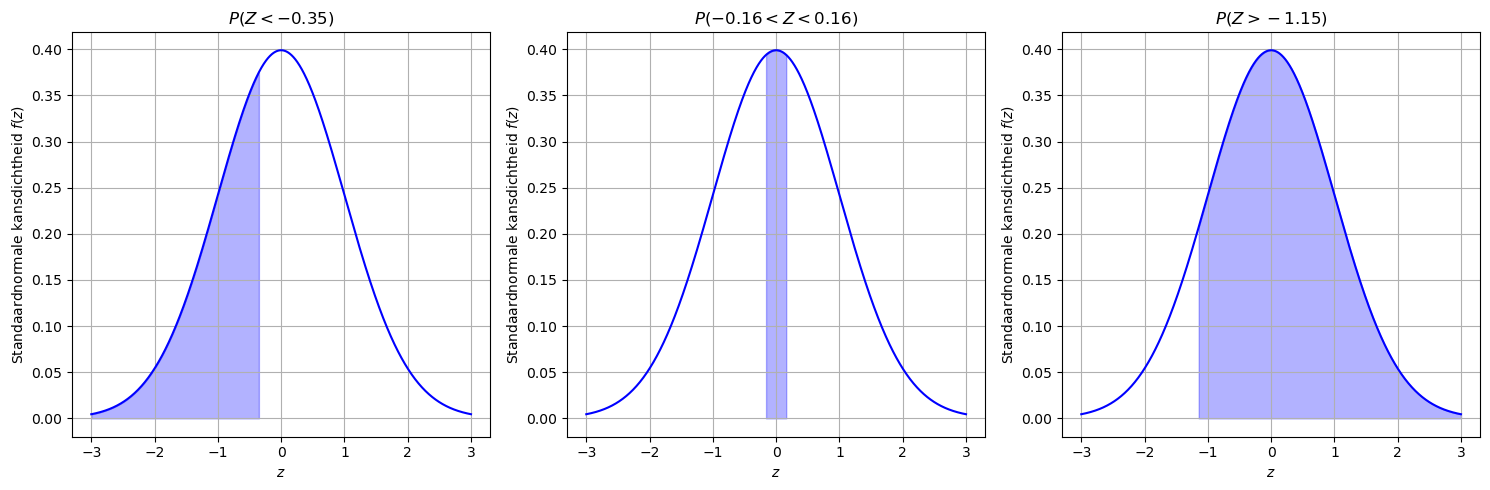
\includegraphics{opg5.4.png}
            }
        \end{center}
}